%%%%%%%%%%%%%%%%%%%%%%%%%%%%%%%%%%%%%%%%%%%%%%%%%%%%%%%%%%%%%%%%%%%%%%%%%%%%%
%
%  System        : 
%  Module        : 
%  Object Name   : $RCSfile$
%  Revision      : $Revision$
%  Date          : $Date$
%  Author        : $Author$
%  Created By    : Robert Heller
%  Created       : Wed May 31 19:37:01 2017
%  Last Modified : <190715.1748>
%
%  Description 
%
%  Notes
%
%  History
% 
%%%%%%%%%%%%%%%%%%%%%%%%%%%%%%%%%%%%%%%%%%%%%%%%%%%%%%%%%%%%%%%%%%%%%%%%%%%%%
%
%    Copyright (C) 2017  Robert Heller D/B/A Deepwoods Software
%			51 Locke Hill Road
%			Wendell, MA 01379-9728
%
%    This program is free software; you can redistribute it and/or modify
%    it under the terms of the GNU General Public License as published by
%    the Free Software Foundation; either version 2 of the License, or
%    (at your option) any later version.
%
%    This program is distributed in the hope that it will be useful,
%    but WITHOUT ANY WARRANTY; without even the implied warranty of
%    MERCHANTABILITY or FITNESS FOR A PARTICULAR PURPOSE.  See the
%    GNU General Public License for more details.
%
%    You should have received a copy of the GNU General Public License
%    along with this program; if not, write to the Free Software
%    Foundation, Inc., 675 Mass Ave, Cambridge, MA 02139, USA.
%
% 
%
%%%%%%%%%%%%%%%%%%%%%%%%%%%%%%%%%%%%%%%%%%%%%%%%%%%%%%%%%%%%%%%%%%%%%%%%%%%%%

\documentclass[12pt,notitlepage,twoside]{book}
\usepackage{graphicx}
\usepackage{mathptm}
\usepackage{times}
\usepackage{makeidx}
\usepackage{ifpdf}
\ifpdf
\usepackage[pdftex,
            pagebackref=true,
            colorlinks=true,
            linkcolor=blue,
            unicode
           ]{hyperref}
\else
\usepackage[ps2pdf,
            pagebackref=true,
            colorlinks=true,
            linkcolor=blue,
            unicode
           ]{hyperref}
\usepackage{pspicture}
\fi
\usepackage{url}
\pagestyle{headings}
\makeindex
\emergencystretch=50pt
\setcounter{tocdepth}{3}
\setcounter{secnumdepth}{3}
\includeonly{SMCSenseHAT,QuadSSSQuadIn,MCP23017,OctalLEDDriver,QuadSMCSenseHat,LCCCANCape,QuadSMCSenseCape,QuadSMCSenseHat}
\begin{document}
\title{Railroad Circuits for the Raspberry Pi, Beagle Bone Black, Pocket Beagle, and ESP32}
\author{Robert Heller \\ The Country Robot \\ Wendell, MA, USA}
\date{\today}
\begin{titlepage}

\maketitle

\clearpage

This documentation was prepared with \LaTeX.

\vspace{.25in}


{\small Copyright \copyright 2017-2019 by Robert Heller D/B/A The Country Robot}
\vspace{.25in}

All rights reserved.  Permission is granted to copy this document in
electronic form only, so long as it is with the software it
documents. 

\vspace{.125in}

The author, Robert Heller, may be contacted electronically (E-Mail) via
\url{mailto:heller@thecountryrobot.com}.

\vspace{.25in}

The Country Robot's web site URL: \url{http://www.thecountryrobot.com/}.

\thispagestyle{empty}
\setcounter{page}{0}
\clearpage

\end{titlepage}

\pagenumbering{roman}
\tableofcontents
\listoffigures
\listoftables
\cleardoublepage
\chapter*{Preface}
\addcontentsline{toc}{chapter}{Preface}

This booklet describes a collection of circuit boards I designed to make use 
of Raspberry Pi GPIO pins to be used in the control of a model railroad 
layout.  I am not formally trained as an electronics engineer, but these 
circuits are fairly simple and are readily cribbed from the data sheets of the 
various microchips used.  If someone who is a trained electronics engineer 
finds something wrong, I would of course like to hear about it.

\cleardoublepage
\pagenumbering{arabic}
\chapter{General Information}

Many of these boards are add on boards for a Raspberry Pi ``B'' model, 
one with a 40-pin header and have the mechanical form factor of a Raspberry Pi 
``HAT''.  Since none of them have an eeprom on them, they are technically not 
actual ``HATs''.  These boards can be ``stacked'', with some limitations, as 
indicated in their respective chapters, mainly because some of these boards 
are hard wired to use specific GPIO pins.  It is therefore possible to use 
``stacking'' (or ``stack through'') headers, headers that are both female 
sockets and male pins.  The end user has a choice of headers to use: standard 
female only headers, long female only headers, standard ``stacking'' headers 
or long/tall ``stacking'' headers.  In the chapters for each board in the 
parts list section, I list the various header options, with part numbers and 
suppliers.  Other boards are stackable ``Capes'' for the Beagle Bone Black. 
Again, since many of these boards are stackable, ``stacking'' (or ``stack 
through'') headers can be used.  Still other boards are for the Pocket Beagle 
and the ESP32 devkit board.  These latter are not meant to be stackable and 
for these, the add on board goes \textit{under} the processor board.  Unlike 
the Raspberry Pi and Beagle Bone Black, these smaller boards have no mounting 
holes, but the ``add on'' boards do.  Also for these smaller boards the add 
on boards provide power to the processor board.

Another place where the end user has choices is in the terminal blocks.  With 
some exceptions (mostly for higher power cases), all of the terminal blocks 
are specified as .1'' (2.54mm) pitch screw terminals.  It is possible to 
substitute other .1'' (2.54mm) pitch connections, including vertical or right 
angle pin arrays or even spring terminals.  This will depend on what sort of 
interconnection technology the end user would prefer.  In the parts list will 
be the various alternative options.

All of the boards use mostly through-hole parts and should be fairly easy to
hand solder with a basic good quality soldering iron. All of the components
are standard and readily available from various suppliers (like Mouser or
Digi-Key).

Most of the boards have mounting holes.  The mounting holes on the HAT-like 
boards align over the mounting holes in the Raspberry Pi.  Using standard 
height headers allows about 3/8'' between boards and using tall headers allows 
1/2'' between boards.  It is probably a good idea to use spacer hardware to 
secure the boards.  Male/female 4-40 threaded hex spacers work quite well, 
although the boards are designed to use M2.5 hardware (Adafruit sells M2.5 
male/female threaded hex spacers in pairs).

%%%%%%%%%%%%%%%%%%%%%%%%%%%%%%%%%%%%%%%%%%%%%%%%%%%%%%%%%%%%%%%%%%%%%%%%%%%%%
%
%  System        : 
%  Module        : 
%  Object Name   : $RCSfile$
%  Revision      : $Revision$
%  Date          : $Date$
%  Author        : $Author$
%  Created By    : Robert Heller
%  Created       : Wed May 31 20:05:00 2017
%  Last Modified : <170531.2005>
%
%  Description 
%
%  Notes
%
%  History
% 
%%%%%%%%%%%%%%%%%%%%%%%%%%%%%%%%%%%%%%%%%%%%%%%%%%%%%%%%%%%%%%%%%%%%%%%%%%%%%
%
%    Copyright (C) 2017  Robert Heller D/B/A Deepwoods Software
%			51 Locke Hill Road
%			Wendell, MA 01379-9728
%
%    This program is free software; you can redistribute it and/or modify
%    it under the terms of the GNU General Public License as published by
%    the Free Software Foundation; either version 2 of the License, or
%    (at your option) any later version.
%
%    This program is distributed in the hope that it will be useful,
%    but WITHOUT ANY WARRANTY; without even the implied warranty of
%    MERCHANTABILITY or FITNESS FOR A PARTICULAR PURPOSE.  See the
%    GNU General Public License for more details.
%
%    You should have received a copy of the GNU General Public License
%    along with this program; if not, write to the Free Software
%    Foundation, Inc., 675 Mass Ave, Cambridge, MA 02139, USA.
%
% 
%
%%%%%%%%%%%%%%%%%%%%%%%%%%%%%%%%%%%%%%%%%%%%%%%%%%%%%%%%%%%%%%%%%%%%%%%%%%%%%

\chapter{SMCSenseHAT: Stall Motor Control and Sense HAT}

%%%%%%%%%%%%%%%%%%%%%%%%%%%%%%%%%%%%%%%%%%%%%%%%%%%%%%%%%%%%%%%%%%%%%%%%%%%%%
%
%  System        : 
%  Module        : 
%  Object Name   : $RCSfile$
%  Revision      : $Revision$
%  Date          : $Date$
%  Author        : $Author$
%  Created By    : Robert Heller
%  Created       : Wed May 31 20:07:09 2017
%  Last Modified : <171103.1610>
%
%  Description 
%
%  Notes
%
%  History
% 
%%%%%%%%%%%%%%%%%%%%%%%%%%%%%%%%%%%%%%%%%%%%%%%%%%%%%%%%%%%%%%%%%%%%%%%%%%%%%
%
%    Copyright (C) 2017  Robert Heller D/B/A Deepwoods Software
%			51 Locke Hill Road
%			Wendell, MA 01379-9728
%
%    This program is free software; you can redistribute it and/or modify
%    it under the terms of the GNU General Public License as published by
%    the Free Software Foundation; either version 2 of the License, or
%    (at your option) any later version.
%
%    This program is distributed in the hope that it will be useful,
%    but WITHOUT ANY WARRANTY; without even the implied warranty of
%    MERCHANTABILITY or FITNESS FOR A PARTICULAR PURPOSE.  See the
%    GNU General Public License for more details.
%
%    You should have received a copy of the GNU General Public License
%    along with this program; if not, write to the Free Software
%    Foundation, Inc., 675 Mass Ave, Cambridge, MA 02139, USA.
%
% 
%
%%%%%%%%%%%%%%%%%%%%%%%%%%%%%%%%%%%%%%%%%%%%%%%%%%%%%%%%%%%%%%%%%%%%%%%%%%%%%

\chapter{QuadSSSQuadIn: Quad SSR and Quad 5V Input HAT}

This is a circuit board to for an add-on board for a Raspberry Pi B+ that will
add four 5V logic inputs and four Solid State Relays, using a MCP23008 I2C I/O 
expander.  There is a jumper header to set one of eight addresses for the 
MCP23008 chip.  This allows using more than one of this board or any other 
board featuring a MCP23008 or MCP23016 or MCP23017 chip (up to eight total).

The circuit board uses a 40pin header socket to connect to the 40pin header on
the  Raspberry Pi B+ and can use a  stack-through  header to allow  additional
boards to be stacked on top of it.

\section{Circuit Description}                                                  
 
\begin{figure}[hbpt]\begin{centering}%
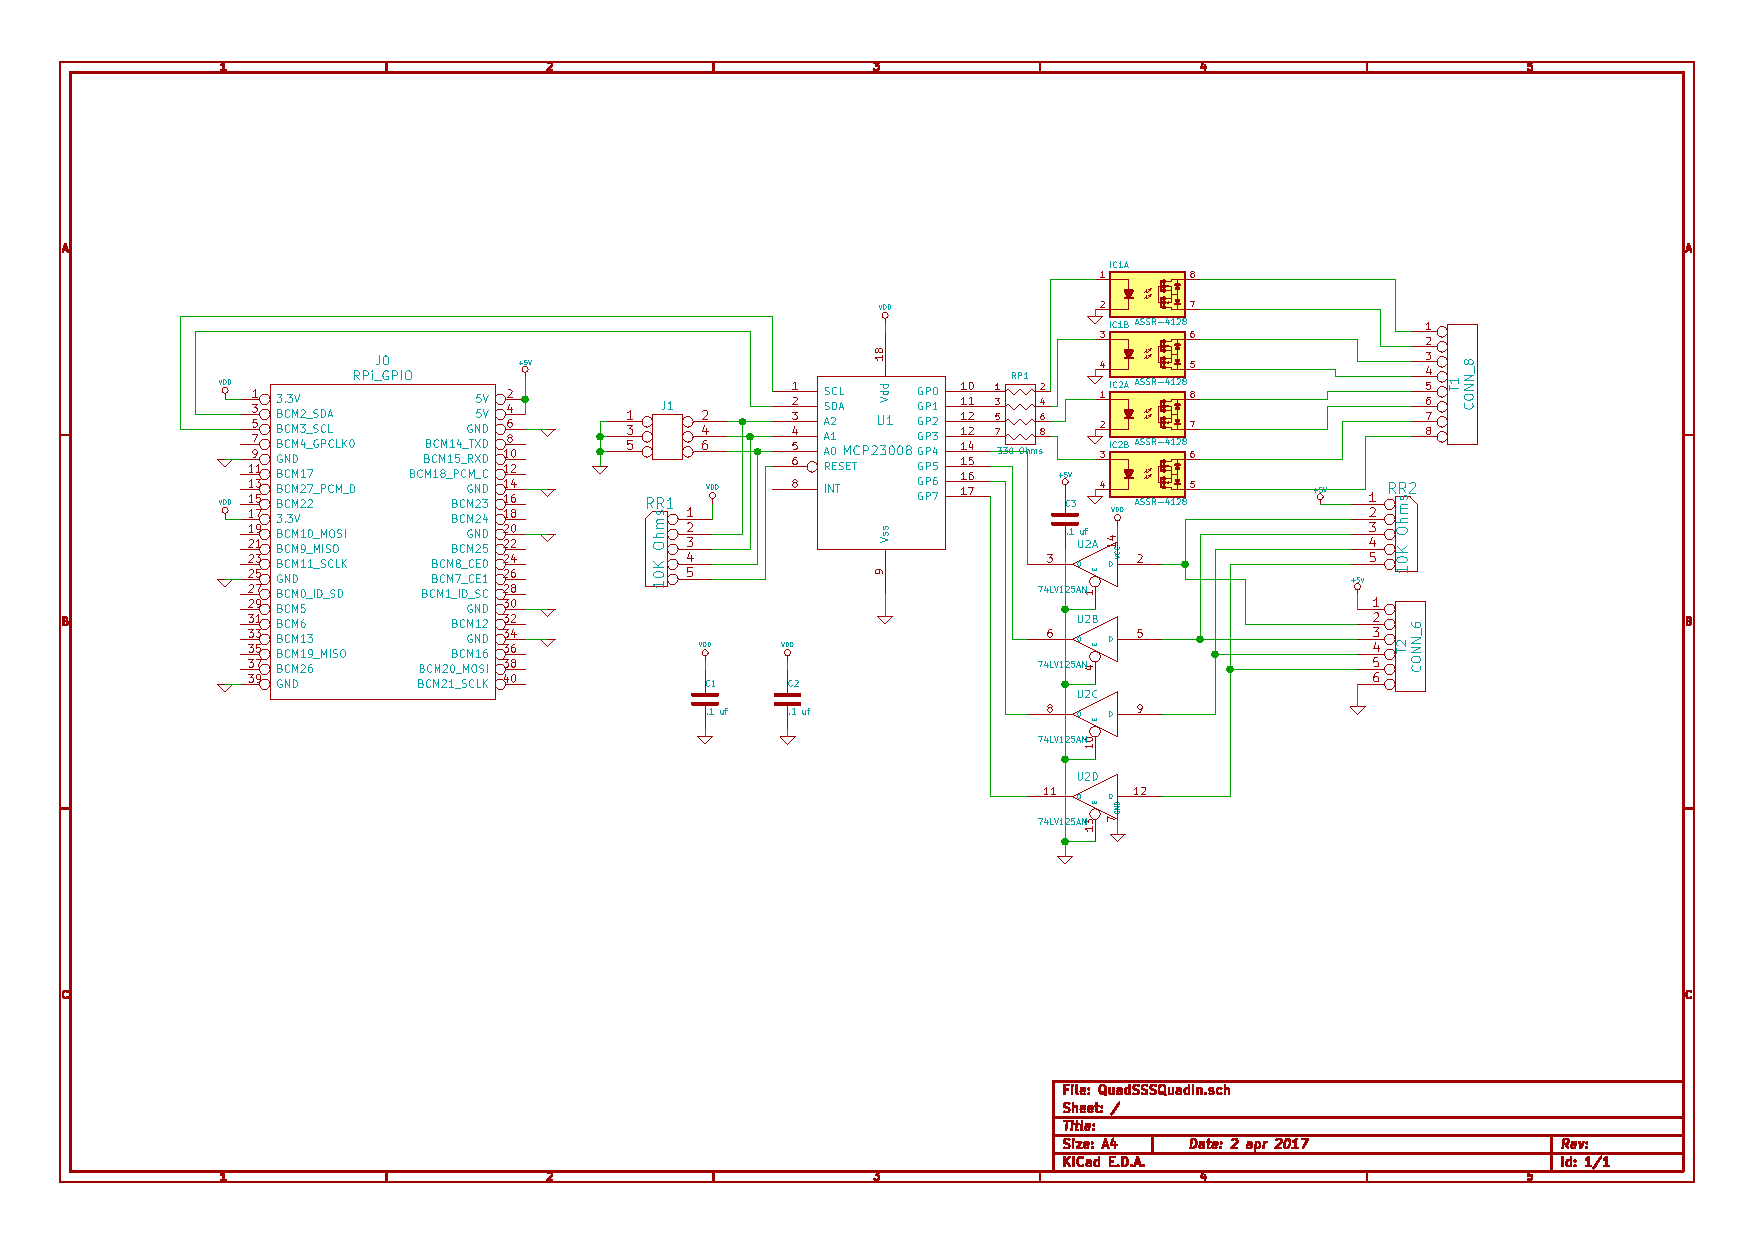
\includegraphics[width=5in]{QuadSSSQuadIn.pdf}
\caption{Circuit Diagram of the QuadSSSQuadIn}
\end{centering}\end{figure}
This circuit uses a MCP23008 to expand the Raspberry Pis I/O to 8 additional 
I/O pins.  Four of these pins (0-3) are used to drive a pair of dual 
opto-isolated SSR chip and the remaining 4 (4-7) are driven by a input buffer 
chip that can be driven with 5V logic.  The SSRs can be used to switch 
arbitrary trackside devices, since the output side of the SSRs are rated upto 
+/- 400 volts at up to 0.1 Amp (100ma).  The 5V logic inputs are compatible 
with many sensor boards available (particularly occupancy detector circuits).

\section{Parts List}

\begin{table}[htdp]
\begin{centering}\begin{tabular}{|l|l|p{1in}|l|p{.5in}|}
\hline
Value&Qty&Refs&Mouser Part Number&Adafruit Part Number\\
\hline
.1 uf&3&C1 C2 C3&21RZ310-RC&\\
\hline
ASSR-4128&2&IC1 IC2&630-ASSR-4128-002E&\\
\hline
RPi GPIO&1&J0&855-M20-6102045&2223\\
\hline
CONN 3X2&1&J1&517-929836-02-03&\\
\hline
330 Ohms&1&RP1&652-4608X-AP2-331LF&\\
\hline
10K Ohms&2&RR1 RR2&652-4605X-1LF-10K&\\
\hline
CONN 8&1&T1&651-1725711&\\
\hline
CONN 6&1&T2&651-1725698&\\
\hline
MCP23008&1&U1&579-MCP23008-E/P&\\
\hline
74LV125AN&1&U2&595-SN74LV125AN&\\
\hline
\end{tabular}
\caption{Parts list for QuadSSSQuadIn boards.}
\end{centering}\end{table}\footnote{Mouser Project link: 
\url{http://www.mouser.com/ProjectManager/ProjectDetail.aspx?AccessID=97fe7b85dc}.}

The only parts that might be substituted are J0 (the RPi GPIO Header), and T1
and T2 (the I/O terminals). The parts listed are for the stacking headers for 
the RPi GPIO Header, and screw terminals for the I/O terminals.  Feel free to 
select a non-stacking header for the RPi GPIO Header and to select either pin 
arrays or spring terminals for the T1 and T2.                   

\section{Circuit Board Layout}

\begin{figure}[hbpt]\begin{centering}%
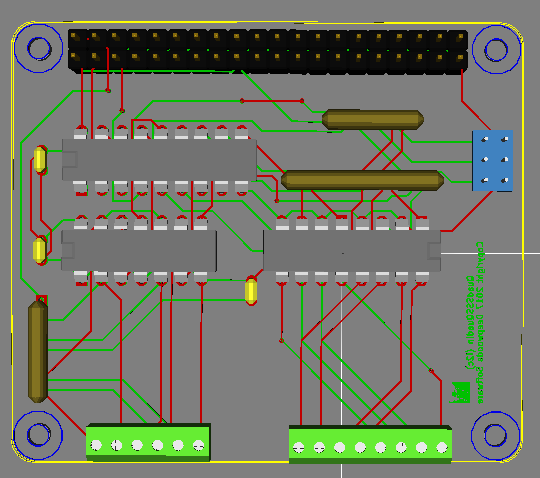
\includegraphics[width=5in]{QuadSSSQuadIn3DTop.png}
\caption{3D rendering of the QuadSSSQuadIn board}
\end{centering}\end{figure}
\begin{figure}[hbpt]\begin{centering}%
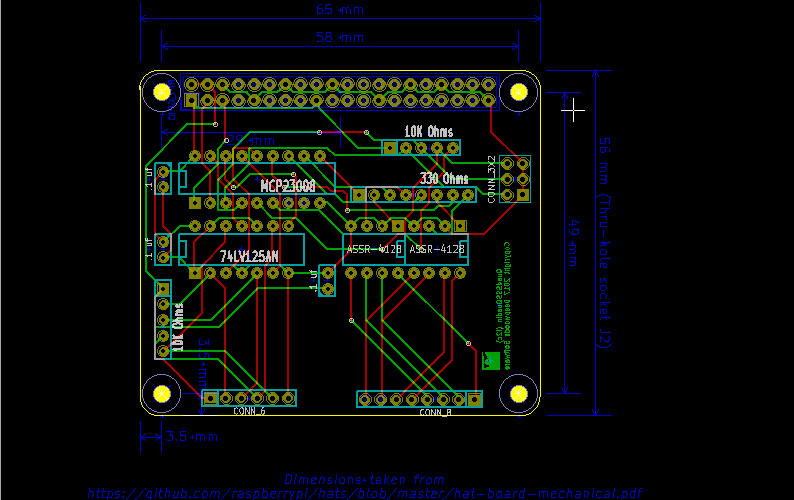
\includegraphics[width=5in]{QuadSSSQuadIn.png}
\caption{Fabrication image of the QuadSSSQuadIn board}
\end{centering}\end{figure}
Board assembly is straight forward.  You need to be careful orienting the ICs, 
noting that the SSRs are oppositely oriented from the other ICs.  Also the 
SIP resistor arrays need to be carefully oriented -- the dot marks pin 1, 
which is indicated on the board with a square pad\footnote{The first batch of 
the boards I ordered used the wrong PCB modules for the terminals and the 
holes are too small for the screw terminal pins to go all the way in.  They 
can be ``jammed'' in enough to be soldered. Pin arrays fit a little better, 
but still need some effort to seat.  The next batch I order will not have this 
problem.}. 


%%%%%%%%%%%%%%%%%%%%%%%%%%%%%%%%%%%%%%%%%%%%%%%%%%%%%%%%%%%%%%%%%%%%%%%%%%%%%
%
%  System        : 
%  Module        : 
%  Object Name   : $RCSfile$
%  Revision      : $Revision$
%  Date          : $Date$
%  Author        : $Author$
%  Created By    : Robert Heller
%  Created       : Wed May 31 20:09:46 2017
%  Last Modified : <170531.2010>
%
%  Description 
%
%  Notes
%
%  History
% 
%%%%%%%%%%%%%%%%%%%%%%%%%%%%%%%%%%%%%%%%%%%%%%%%%%%%%%%%%%%%%%%%%%%%%%%%%%%%%
%
%    Copyright (C) 2017  Robert Heller D/B/A Deepwoods Software
%			51 Locke Hill Road
%			Wendell, MA 01379-9728
%
%    This program is free software; you can redistribute it and/or modify
%    it under the terms of the GNU General Public License as published by
%    the Free Software Foundation; either version 2 of the License, or
%    (at your option) any later version.
%
%    This program is distributed in the hope that it will be useful,
%    but WITHOUT ANY WARRANTY; without even the implied warranty of
%    MERCHANTABILITY or FITNESS FOR A PARTICULAR PURPOSE.  See the
%    GNU General Public License for more details.
%
%    You should have received a copy of the GNU General Public License
%    along with this program; if not, write to the Free Software
%    Foundation, Inc., 675 Mass Ave, Cambridge, MA 02139, USA.
%
% 
%
%%%%%%%%%%%%%%%%%%%%%%%%%%%%%%%%%%%%%%%%%%%%%%%%%%%%%%%%%%%%%%%%%%%%%%%%%%%%%

\chapter{MCP23017Hat: 16 bit GPIO expander HAT}

%%%%%%%%%%%%%%%%%%%%%%%%%%%%%%%%%%%%%%%%%%%%%%%%%%%%%%%%%%%%%%%%%%%%%%%%%%%%%
%
%  System        : 
%  Module        : 
%  Object Name   : $RCSfile$
%  Revision      : $Revision$
%  Date          : $Date$
%  Author        : $Author$
%  Created By    : Robert Heller
%  Created       : Fri Nov 3 11:46:41 2017
%  Last Modified : <171103.2143>
%
%  Description 
%
%  Notes
%
%  History
% 
%%%%%%%%%%%%%%%%%%%%%%%%%%%%%%%%%%%%%%%%%%%%%%%%%%%%%%%%%%%%%%%%%%%%%%%%%%%%%
%
%    Copyright (C) 2017  Robert Heller D/B/A Deepwoods Software
%			51 Locke Hill Road
%			Wendell, MA 01379-9728
%
%    This program is free software; you can redistribute it and/or modify
%    it under the terms of the GNU General Public License as published by
%    the Free Software Foundation; either version 2 of the License, or
%    (at your option) any later version.
%
%    This program is distributed in the hope that it will be useful,
%    but WITHOUT ANY WARRANTY; without even the implied warranty of
%    MERCHANTABILITY or FITNESS FOR A PARTICULAR PURPOSE.  See the
%    GNU General Public License for more details.
%
%    You should have received a copy of the GNU General Public License
%    along with this program; if not, write to the Free Software
%    Foundation, Inc., 675 Mass Ave, Cambridge, MA 02139, USA.
%
% 
%
%%%%%%%%%%%%%%%%%%%%%%%%%%%%%%%%%%%%%%%%%%%%%%%%%%%%%%%%%%%%%%%%%%%%%%%%%%%%%

\chapter{OctalLEDDriver: Octal LED (Common Cathode) driver board.}

This is a standalone board that takes 8 3V GPIO pins (such as from a MCP23017 
or MCP23008 HAT board or just from 8 of a Raspberry Pi's GPIO pins and buffers 
them to drive up to 8 LEDs from a 5V supply.  It is specificly designed for 
common cathode signals.  It has a ten position screw terminal at one end, for 
GND, GPIO 0 through 7, and +3V (it does not actually use the +3V connection, 
but includes it to match the terminals on a MCP23017 or MCP23008 HAT board and 
thus can support the use of ten conductor cable or pin header connectors, 
etc.).  At the other end it is two sets of +5V and ground terminals (to allow 
for daisy chaining the +5V supply bus), and nine position screw terminal for 
LEDs 0 though 7 and the common cathode (K), which is ground.

\section{Circuit Description}

\begin{figure}[hbpt]\begin{centering}%
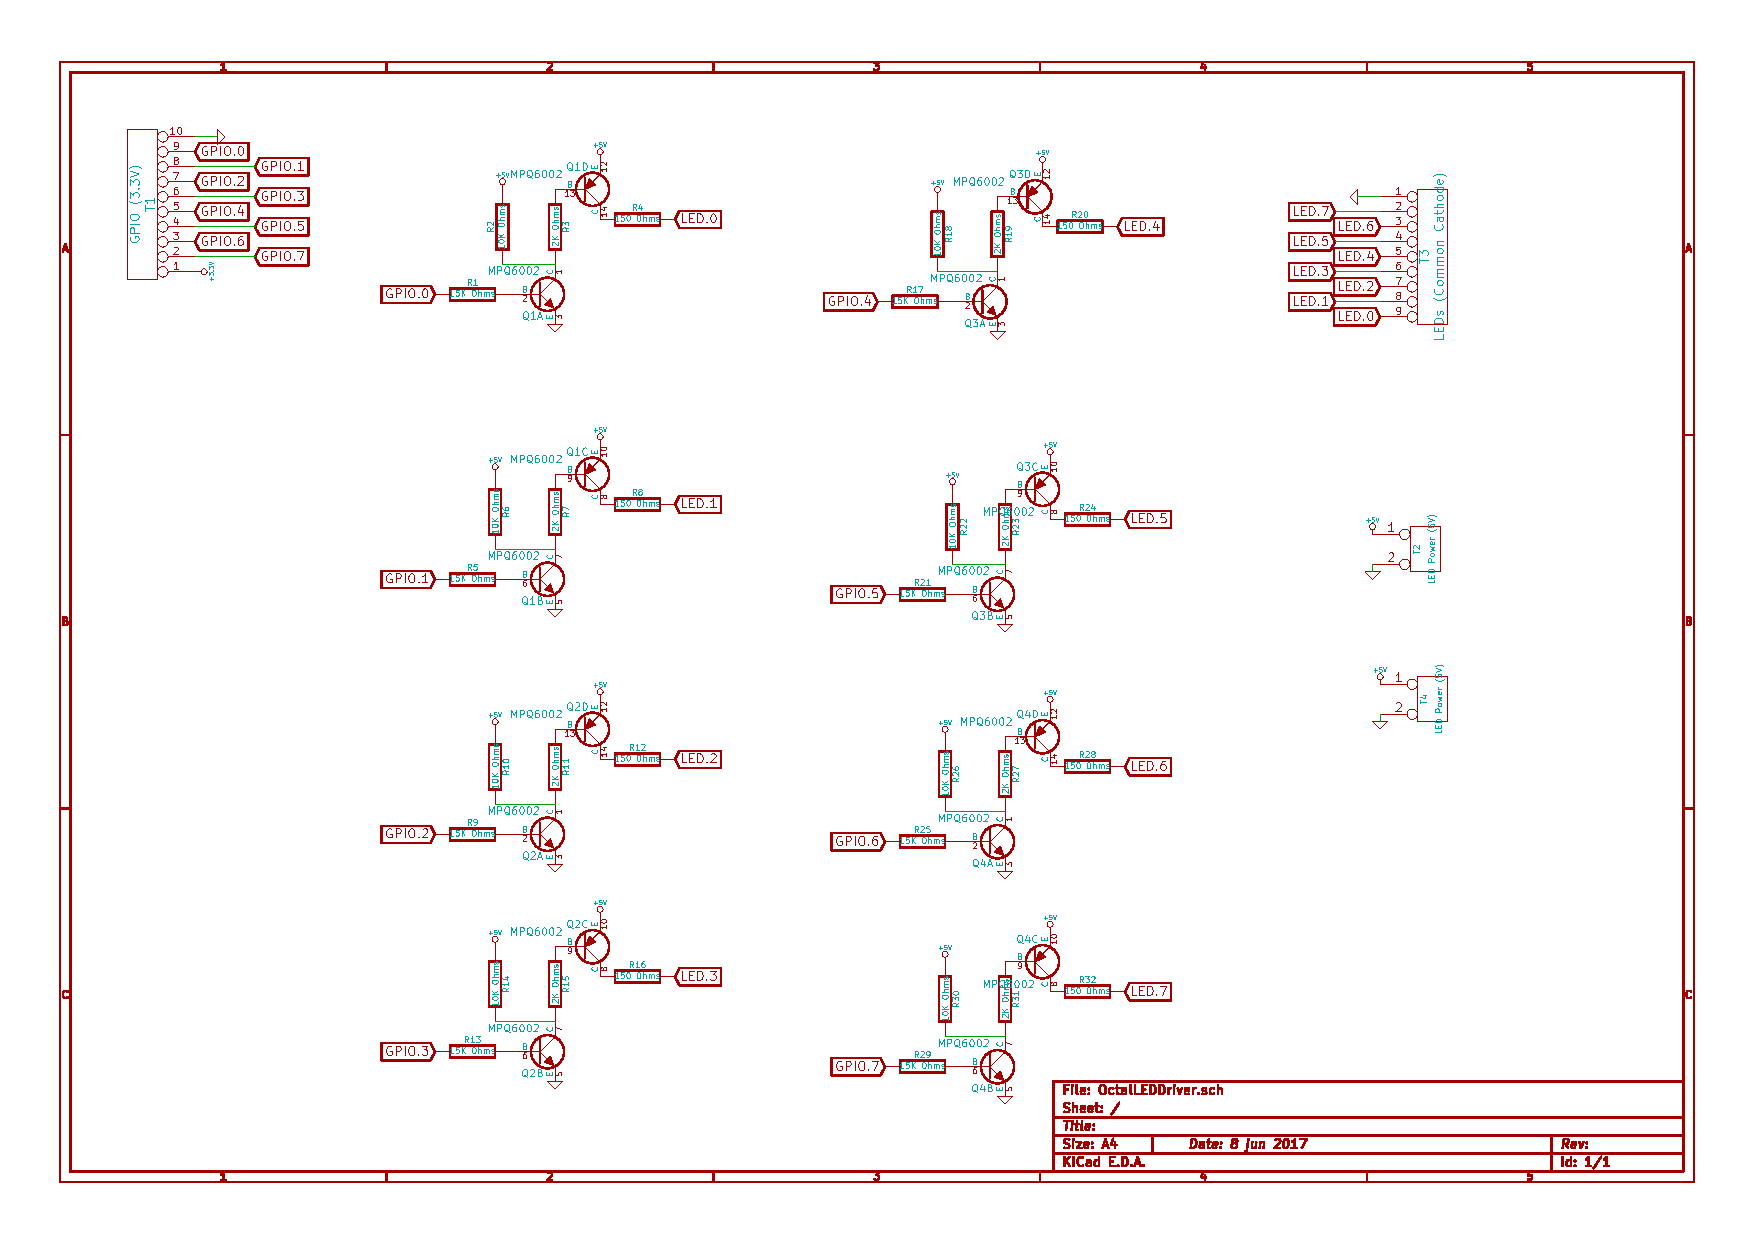
\includegraphics[width=5in]{OctalLEDDriver.pdf}
\caption{Circuit Diagram of the OctalLEDDriver}
\end{centering}\end{figure}
The circuit is just eight driver circuits, each featuring a NPN and a PNP 
transistor, that level shift and buffer the 3V logic to 20 milliamp, 5V LED 
drive circuits.  The circuits include a current limiting series resistor, so 
there is no need to include resistors.  The circuit assumes 2V LEDs (typical 
of standard red, green, and yellow LEDs).

\section{Parts List}

\begin{table}[htdp]
\begin{centering}\begin{tabular}{|l|l|p{1in}|l|}
\hline
Value&Quantity&References&Mouser Part Number\\
\hline
MPQ6002&4&Q1 Q2 Q3 Q4&610-MPQ6002\\
\hline
15K Ohms&8&R1 R5 R9 R13 R17 R21 R25 R29&603-CFR-25JR-5215K\\
\hline
10K Ohms&8&R2 R6 R10 R14 R18 R22 R26 R30&603-CFR-25JR-5210K\\
\hline
2K Ohms&8&R3 R7 R11 R15 R19 R23 R27 R31&603-CFR-25JR-522K\\
\hline
150 Ohms&8&R4 R8 R12 R16 R20 R24 R28 R32&588-OK1515E-R52\\
\hline
GPIO (3.3V)&1&T1&651-1725737 or 2x 651-1725685 \\
\hline
LED Power (5V)&2&T2 T4&651-1725656\\
\hline
LEDs (Common Cathode)&1&T3&651-1725724\\
\hline
\end{tabular}
\caption{Parts list for OctalLEDDriver boards.}
\end{centering}\end{table}\footnote{Mouser Project link: 
\url{http://www.mouser.com/ProjectManager/ProjectDetail.aspx?AccessID=f337ca3247}.}

The only parts that might be substituted are the screw terminal boards. Feel 
free to select either pin arrays or spring terminals for the terminals.

\section{Circuit Board Layout}

\begin{figure}[hbpt]\begin{centering}%
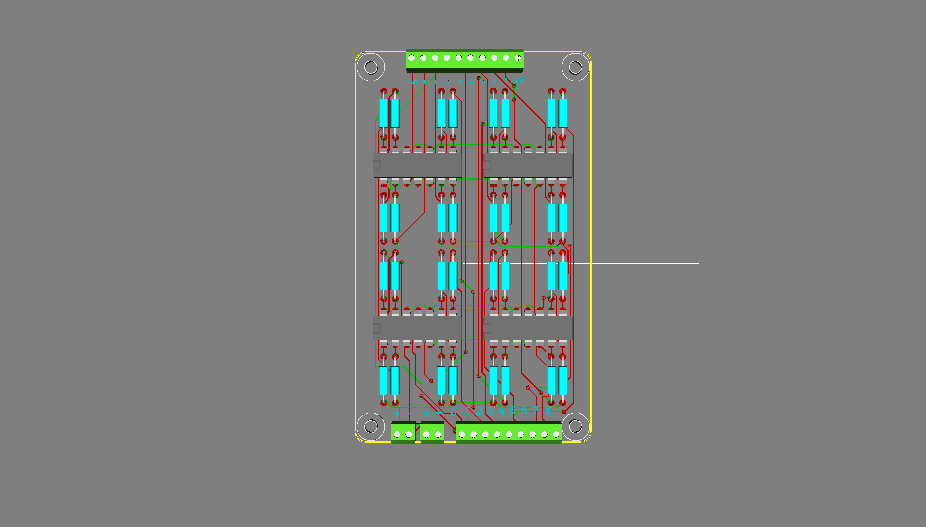
\includegraphics[width=5in]{OctalLEDDriver3DTop.png}
\caption{3D rendering of the OctalLEDDriver board}
\end{centering}\end{figure}
\begin{figure}[hbpt]\begin{centering}%
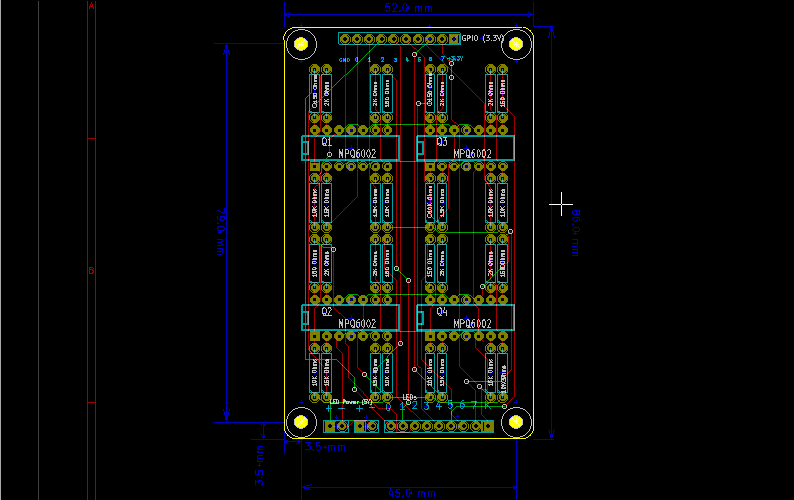
\includegraphics[width=5in]{OctalLEDDriver.png}
\caption{Fabrication image of the OctalLEDDriver board}
\end{centering}\end{figure}
Board assembly is straight forward. You need to be careful orienting the quad 
transistors. 

\section{Downloadables}

Full design information is available on GitHub here:
\url{https://github.com/RobertPHeller/RPi-RRCircuits/tree/master/OctalLEDDriver}.




../QuadSMCSenseHat/QuadSMCSenseHat.tex
%%%%%%%%%%%%%%%%%%%%%%%%%%%%%%%%%%%%%%%%%%%%%%%%%%%%%%%%%%%%%%%%%%%%%%%%%%%%%
%
%  System        : 
%  Module        : 
%  Object Name   : $RCSfile$
%  Revision      : $Revision$
%  Date          : $Date$
%  Author        : $Author$
%  Created By    : Robert Heller
%  Created       : Mon Jul 15 17:34:14 2019
%  Last Modified : <220902.0854>
%
%  Description 
%
%  Notes
%
%  History
% 
%%%%%%%%%%%%%%%%%%%%%%%%%%%%%%%%%%%%%%%%%%%%%%%%%%%%%%%%%%%%%%%%%%%%%%%%%%%%%
%
%    Copyright (C) 2019  Robert Heller D/B/A Deepwoods Software
%			51 Locke Hill Road
%			Wendell, MA 01379-9728
%
%    This program is free software; you can redistribute it and/or modify
%    it under the terms of the GNU General Public License as published by
%    the Free Software Foundation; either version 2 of the License, or
%    (at your option) any later version.
%
%    This program is distributed in the hope that it will be useful,
%    but WITHOUT ANY WARRANTY; without even the implied warranty of
%    MERCHANTABILITY or FITNESS FOR A PARTICULAR PURPOSE.  See the
%    GNU General Public License for more details.
%
%    You should have received a copy of the GNU General Public License
%    along with this program; if not, write to the Free Software
%    Foundation, Inc., 675 Mass Ave, Cambridge, MA 02139, USA.
%
% 
%
%%%%%%%%%%%%%%%%%%%%%%%%%%%%%%%%%%%%%%%%%%%%%%%%%%%%%%%%%%%%%%%%%%%%%%%%%%%%%

\chapter{LCCCANCape: LCC CAN Tranceiver Cape}

\section{GPIO Pins Used and stacking restrictions.}

This board uses two pins on header P9: 24 and 26 in pin mux mode2, which makes 
pin 24 Can1 RX, and pin 26 Can1 TX.  Only one of these capes can be on any 
Beagle Bone Black.


\section{Circuit Description}

\begin{figure}[hbpt]\begin{centering}%                                         
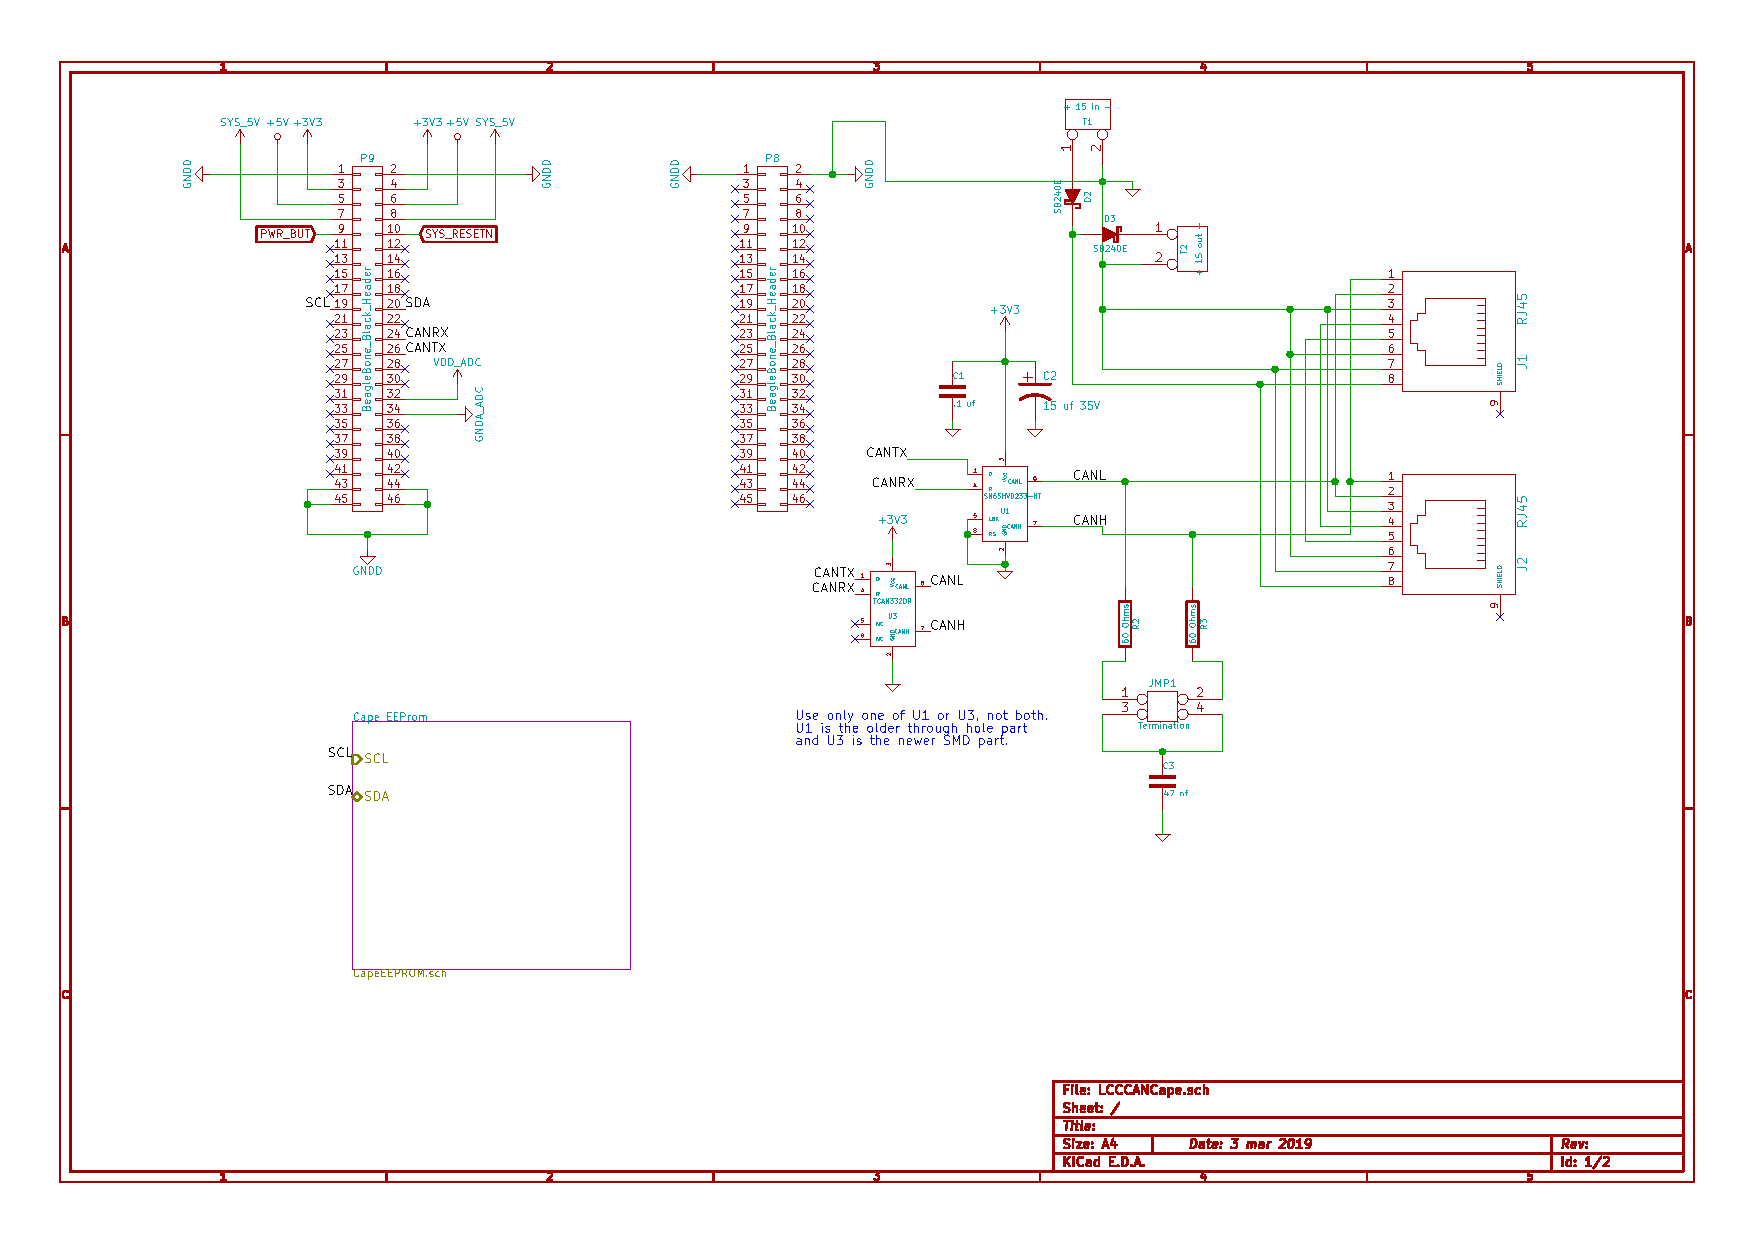
\includegraphics[width=5in]{LCCCANCape-1.pdf}                               
\caption{Circuit Diagram of the LCCCANCape}                               
\end{centering}\end{figure}                                                    
This circuit contains two sectins.  There is the transciever section, which 
includes the transciver itself, the termination block, the two RJ45 jacks, and 
two terminal blocks for injecting and tapping into the power carried in the 
CAT 5 cable.  Power is not used to power the Beagle Bone Black.  The other 
section is the Cape EErom circuit.  The Cape EEProm contains         
information about the cape and the name and version of the overlay that needs  
to be loaded by uBoot.  

\clearpage

\section{Parts List}

\begin{table}[htp]
\begin{centering}\begin{tabular}{|l|l|p{1in}|l|}
\hline
Value&Quantity&References&Mouser Part Number \\
\hline
.1 uf&1&C8&581-SR201C104KARTR1 \\
\hline
WP 1 0&1&P2&649-67996-406HLF \\
\hline
5.6K Ohms&2&R3 R4&603-CFR-25JR-525K6 \\
\hline
4.75K Ohms&3&R5 R6 R7&603-CFR-25JR-524K7 \\
\hline
10K Ohms&1&R8&603-CFR-25JR-5210K \\
\hline
CAT24C256W&1&U9&698-CAT24C256WI-GT3 \\
\hline
.1 uf&1&C1&21RZ310-RC \\
\hline
15 uf 63V&1&C2&710-860080773002 \\
\hline
47 nf&1&C3&75-1C10Z5U473M050B \\
\hline
SB240E&2&D1 D2&625-SB240-E3 \\
\hline
RJ45&2&J1 J2&710-615008144221 \\
\hline
Termination&1&JP1&649-67997-404HLF \\
\hline
60 Ohms&2&R1 R2&71-RN60C60R0B/R \\
\hline
+ 15 in -;+ 15 out -&2&T1 T2&651-1725656 \\
\hline
TCAN332DR&1&U1&595-TCAN332DR \\
\hline
SN65HVD233-HT&1&U2&595-SN65HVD233SJD \\
\hline
BeagleBone\_Black\_Header&2&''P8 P9''&200-ESQ12314GD \\
\hline
\end{tabular}
\caption{Parts list for LCCCANCape board.}
\end{centering}\end{table}\footnote{Mouser Project links: 
\url{http://www.mouser.com/ProjectManager/ProjectDetail.aspx?AccessID=ae58a2d985},
\url{http://www.mouser.com/ProjectManager/ProjectDetail.aspx?AccessID=522a1259b2}.}


The only parts that might be substituted are P8 and P9 (the Beagle Bone Black
Headers). The parts listed are for the stacking headers for the Beagle Bone
Black Headers. Feel free to select a non-stacking header for the Beagle Bone
Black Headers.


\section{Circuit Board Layout}

\begin{figure}[hbpt]\begin{centering}%
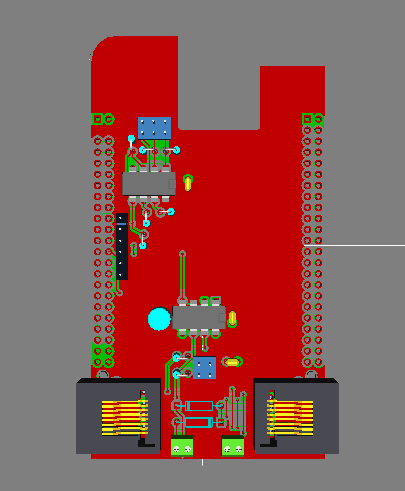
\includegraphics[height=7in]{LCCCANCape3DTop.png}
\caption{3D rendering of the LCCCANCape board}
\end{centering}\end{figure}
\begin{figure}[hbpt]\begin{centering}%
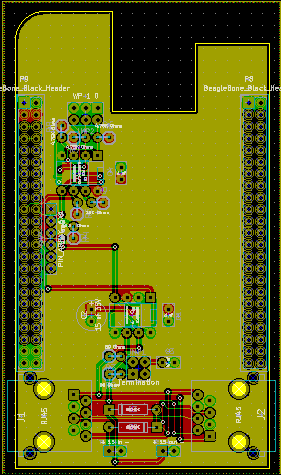
\includegraphics[height=7in]{LCCCANCape.png}
\caption{Fabrication image of the LCCCANCape board}
\end{centering}\end{figure}
Board assembly is straight forward. You need to be careful orienting the ICs
and the electrolytic capacitor.


\section{Downloadables and Software Support}

Full design information is available on GitHub here:
\url{https://github.com/RobertPHeller/RPi-RRCircuits/tree/master/LCCCANCape}.

This board is supported by both the Model Railroad System 
(\url{https://github.com/RobertPHeller/ModelRRSystem}) and the OpenMRN 
(\url{https://github.com/bakerstu/openmrn}).

%%%%%%%%%%%%%%%%%%%%%%%%%%%%%%%%%%%%%%%%%%%%%%%%%%%%%%%%%%%%%%%%%%%%%%%%%%%%%
%
%  System        : 
%  Module        : 
%  Object Name   : $RCSfile$
%  Revision      : $Revision$
%  Date          : $Date$
%  Author        : $Author$
%  Created By    : Robert Heller
%  Created       : Mon Jul 15 17:33:37 2019
%  Last Modified : <190715.1733>
%
%  Description 
%
%  Notes
%
%  History
% 
%%%%%%%%%%%%%%%%%%%%%%%%%%%%%%%%%%%%%%%%%%%%%%%%%%%%%%%%%%%%%%%%%%%%%%%%%%%%%
%
%    Copyright (C) 2019  Robert Heller D/B/A Deepwoods Software
%			51 Locke Hill Road
%			Wendell, MA 01379-9728
%
%    This program is free software; you can redistribute it and/or modify
%    it under the terms of the GNU General Public License as published by
%    the Free Software Foundation; either version 2 of the License, or
%    (at your option) any later version.
%
%    This program is distributed in the hope that it will be useful,
%    but WITHOUT ANY WARRANTY; without even the implied warranty of
%    MERCHANTABILITY or FITNESS FOR A PARTICULAR PURPOSE.  See the
%    GNU General Public License for more details.
%
%    You should have received a copy of the GNU General Public License
%    along with this program; if not, write to the Free Software
%    Foundation, Inc., 675 Mass Ave, Cambridge, MA 02139, USA.
%
% 
%
%%%%%%%%%%%%%%%%%%%%%%%%%%%%%%%%%%%%%%%%%%%%%%%%%%%%%%%%%%%%%%%%%%%%%%%%%%%%%


\cleardoublepage
%\bibliography{MRR}
%\bibliographystyle{plain}
\cleardoublepage
\printindex
\end{document}
